\documentclass[dvipsnames]{beamer}\usepackage[]{graphicx}\usepackage[]{color}
%% maxwidth is the original width if it is less than linewidth
%% otherwise use linewidth (to make sure the graphics do not exceed the margin)
\makeatletter
\def\maxwidth{ %
  \ifdim\Gin@nat@width>\linewidth
    \linewidth
  \else
    \Gin@nat@width
  \fi
}
\makeatother

\definecolor{fgcolor}{rgb}{0.345, 0.345, 0.345}
\newcommand{\hlnum}[1]{\textcolor[rgb]{0.686,0.059,0.569}{#1}}%
\newcommand{\hlstr}[1]{\textcolor[rgb]{0.192,0.494,0.8}{#1}}%
\newcommand{\hlcom}[1]{\textcolor[rgb]{0.678,0.584,0.686}{\textit{#1}}}%
\newcommand{\hlopt}[1]{\textcolor[rgb]{0,0,0}{#1}}%
\newcommand{\hlstd}[1]{\textcolor[rgb]{0.345,0.345,0.345}{#1}}%
\newcommand{\hlkwa}[1]{\textcolor[rgb]{0.161,0.373,0.58}{\textbf{#1}}}%
\newcommand{\hlkwb}[1]{\textcolor[rgb]{0.69,0.353,0.396}{#1}}%
\newcommand{\hlkwc}[1]{\textcolor[rgb]{0.333,0.667,0.333}{#1}}%
\newcommand{\hlkwd}[1]{\textcolor[rgb]{0.737,0.353,0.396}{\textbf{#1}}}%

\usepackage{framed}
\makeatletter
\newenvironment{kframe}{%
 \def\at@end@of@kframe{}%
 \ifinner\ifhmode%
  \def\at@end@of@kframe{\end{minipage}}%
  \begin{minipage}{\columnwidth}%
 \fi\fi%
 \def\FrameCommand##1{\hskip\@totalleftmargin \hskip-\fboxsep
 \colorbox{shadecolor}{##1}\hskip-\fboxsep
     % There is no \\@totalrightmargin, so:
     \hskip-\linewidth \hskip-\@totalleftmargin \hskip\columnwidth}%
 \MakeFramed {\advance\hsize-\width
   \@totalleftmargin\z@ \linewidth\hsize
   \@setminipage}}%
 {\par\unskip\endMakeFramed%
 \at@end@of@kframe}
\makeatother

\definecolor{shadecolor}{rgb}{.97, .97, .97}
\definecolor{messagecolor}{rgb}{0, 0, 0}
\definecolor{warningcolor}{rgb}{1, 0, 1}
\definecolor{errorcolor}{rgb}{1, 0, 0}
\newenvironment{knitrout}{}{} % an empty environment to be redefined in TeX

\usepackage{alltt}
\usepackage{color} % for colors
\usepackage{graphicx}
\usepackage{hyperref}
\usepackage{multicol}
\usepackage{dirtytalk} % this is for the say{} below (i.e.\ the quote)
\usepackage{svg}
\hypersetup{
    bookmarks=true,         % show bookmarks bar?
    unicode=false,          % non-Latin characters in Acrobat?s bookmarks
    pdftoolbar=true,        % show Acrobat?s toolbar?
    pdfmenubar=true,        % show Acrobat?s menu?
    pdffitwindow=false,     % window fit to page when opened
    pdfstartview={FitH},    % fits the width of the page to the window
    pdftitle={My title},    % title
    pdfauthor={Author},     % author
    pdfsubject={Subject},   % subject of the document
    pdfcreator={Creator},   % creator of the document
    pdfproducer={Producer}, % producer of the document
    pdfkeywords={keyword1} {key2} {key3}, % list of keywords
    pdfnewwindow=true,      % links in new PDF window
    colorlinks=true,       % false: boxed links; true: colored links
    linkcolor=red,          % color of internal links (change box color with linkbordercolor)
    citecolor=green,        % color of links to bibliography
    filecolor=magenta,      % color of file links
    urlcolor=blue         % color of external links
}
% \usepackage{beamerthemesplit} // Activate for custom appearance
\beamertemplatenavigationsymbolsempty

\definecolor{wapurple}{HTML}{433447}
\definecolor{wared}{HTML}{D16B54}

\usecolortheme{beaver}
\title{E-411-PRMA}
\subtitle{Lecture 6}
\author{Christopher David Desjardins}
\date{3 September 2015}
\IfFileExists{upquote.sty}{\usepackage{upquote}}{}
\begin{document}





\frame{\titlepage}

\begin{frame}
\frametitle{Standard Error Measurement}
$$\sigma_{SEM} = \sigma\sqrt{1 - r_{xx}}$$
\begin{itemize}
\item standard error of measurement = standard deviation of test scores * square root of 1 - reliability coefficient of the test
  \item<2->Can use this to create confidence intervals by using normality assumption of an individual's score on a large number of tests centered at the mean
  \item<2-> Determines the range of plausible values for a person's true score
\end{itemize}
\end{frame}

\begin{frame}
\frametitle{SEM example}

A math test is administered. The test scores have a reliability of 0.80 and a standard deviation of 0.5

\vspace{1cm}
What is the standard error of measurement?

\vspace{1cm}
If Anna scored a 7.5, what range of values can we be 95\% confident that her true score lies between? 99\% confident?
\end{frame}

\begin{frame}
\frametitle{Standard Error of the difference between two scores}
$$\sigma_D = \sqrt{\sigma_{SEM_1} + \sigma_{SEM_2}} $$

$$\sigma_D = \sigma\sqrt{2 - r_1 - r_2} $$

\begin{itemize}
  \item Can be used to compare two individuals on the same test or a different test
  \item Can be used to compare performance of an individual on two tests
\end{itemize}
\end{frame}

\begin{frame}
\frametitle{SED example}
Sigrun takes the same test as Anna and scores a 6.5. Did Anna perform significantly better on the test? 

\vspace{1cm}
If Anna took a second test and got a score of 8 and the reliability coefficient for the second test was 0.6, did Anna do significantly better on the second test?

\end{frame}

{
\setbeamercolor{normal text}{bg=blue}
\begin{frame}
\centering\Huge \textcolor{white}{Validity}
\end{frame}
}

\frame
{
  \frametitle{Validity}

  \begin{itemize}
  	\item What is validity?
		\begin{itemize}
			\item An indicator of how well the test measures the latent construct(s) it claims to.
			\item A determination of the appropriateness of the test scores for specific uses/users 	
			\item Validity of the test for a \textcolor{red}{given purpose, at a given time, for a given population}
			\item You are a lawyer presenting evidence to a judge to make the case for the validity of your instrument - \textcolor{red}{validation}
			\item Users can conduct a \textcolor{red}{validation study} to assess the validity of the instrument for their purposes
		\end{itemize}  
  \end{itemize}
}

\frame{
\frametitle{Overview of Validity}
\begin{itemize}
	\item \textcolor{wapurple}{Content} - Evaluation of the subjects, topic, or content \textcolor{wared}{covered by the items in the test}
	\item \textcolor{wapurple}{Criterion-Related} - \textcolor{wared}{Evaluating the relationship} of scores obtained on the test to scores on other tests or measures
	\item \textcolor{wapurple}{Construct} - \textcolor{wared}{Evaluation} of how scores obtained on the test relate to scores on other instruments \textcolor{wared}{AND} understanding how the test scores fit within the \textcolor{wared}{theoretical framework of the latent construct} that the test purports to measure
	\end{itemize}
}

\frame{
\frametitle{Content Validity}
\begin{itemize}
	\item How adequately the test represents the latent construct of interest
	\item Do the items throughly and completely tap into the latent construct?
	\item Content valid test would have percentage of items on each topics to be proportional to the amount of time spent on these topics
	\item \textcolor{wapurple}{How can we be sure I am teaching the entire domain of psychological testing?}
	\item Create a \textcolor{wared}{test blueprint} 
		\begin{itemize}
			\item What could be conceivably measured and in what proportion
			\item Number of questions, types of questions, areas covered, organization, etc
		\end{itemize}
\end{itemize}
}

\frame{
\frametitle{Assessing Content Validity}
\begin{itemize}
	\item Assume you are giving an instrument to measure aggressive behavior in children
	\item \textcolor{wapurple}{How can we assume this is measuring the construct of aggression quantitatively?}
		\begin{itemize}
			\item Experts assess whether each item is essential, useful, or not necessary to the definition of aggression
			\item $CVR = \frac{n_e - (N / 2)}{N / 2}$
			\item Where $n_e$ is number say ``essential" and N is number of experts
			\item Want this larger than chance (Table 6-1)
		\end{itemize}	 
\end{itemize}
}

\begin{frame}[fragile]
\frametitle{CVR in toy example}
\begin{itemize}
\item "Does your child bite other children?"
\item 20 experts, 17 say ``essential"
\end{itemize}
\end{frame}

\begin{frame}[fragile]
\frametitle{Letting R do the work}
\begin{knitrout}
\definecolor{shadecolor}{rgb}{0.969, 0.969, 0.969}\color{fgcolor}\begin{kframe}
\begin{alltt}
\hlstd{CVR} \hlkwb{<-} \hlkwa{function}\hlstd{(}\hlkwc{n}\hlstd{,} \hlkwc{essential}\hlstd{)\{}
  \hlstd{(essential} \hlopt{-} \hlstd{n}\hlopt{/}\hlnum{2}\hlstd{)}\hlopt{/}\hlstd{(n}\hlopt{/}\hlnum{2}\hlstd{)}
\hlstd{\}}
\hlkwd{CVR}\hlstd{(}\hlkwc{n} \hlstd{=} \hlnum{20}\hlstd{,} \hlkwc{essential} \hlstd{=} \hlnum{17}\hlstd{)}
\end{alltt}
\begin{verbatim}
## [1] 0.7
\end{verbatim}
\end{kframe}
\end{knitrout}
\end{frame}

\frame{
\frametitle{Assessing Content Validity}

\begin{center}
{\huge BUT ... expert judgement!!!}
\end{center}
}

\frame{
\say{Who controls the past controls the future; who controls the present controls the past.}

\vspace{1cm}
\centerline{
\includegraphics[scale=.5]{images/orwell.jpg}}

\vfill
{\footnotesize \href{https://c2.staticflickr.com/4/3463/3730530834_31d8f32a3b.jpg}{source}}
}

\frame{
\frametitle{Criterion-Related Validity}
\begin{itemize}
	\item What the test score tells you about where a person falls on the underlying construct being measured w.r.t a criterion 
	\item  A \textcolor{wared}{criterion} is a benchmark or standard used for comparison
	\item Scores on a new IQ instrument, \textit{but do you really know that high scores mean high IQ}?
	  \begin{itemize}
	    \item Should be \textcolor{wared}{relevant}
	    \begin{itemize}
	    \item People that are known to have high IQs (maybe MENSA membership) should score highly on this instrument 
	    \end{itemize}
	    \item Should be \textcolor{wared}{valid} for measuring IQ
	    \begin{itemize}
	      \item Who created this instrument?
	      \item Does it correlate with established IQ instruments (e.g.\ WAIS or Stanford-Binet)?
	  \end{itemize}
\end{itemize}
\end{itemize}
}



\frame{
\frametitle{Criterion Problems}
\begin{itemize}
	\item Predict whether someone is receiving counseling services based on Beck Depression Inventory
	  \begin{itemize}
	\item Find out BDI was used to determine whether someone should receive services
	  \end{itemize}
	  \item <2->In addition, to self-report and parent report, you ask teachers to rate students on externalizing behaviors
	  \begin{itemize}
	    \item <2-> After all the students' scores have been calculated, ask teachers to comment on them
	  \end{itemize}
	\item<3-> \textcolor{wared}{What is wrong with this?} 
\end{itemize}
}

\frame{
\frametitle{Concurrent Validity}
\begin{itemize}
\item \textcolor{wapurple}{Concurrent Validity}
\begin{itemize}
	  \item Test scores are obtained at the \textit{same time} as the criterion measures are obtained
	  \item Measures of the relationship between the test and the criterion are \textcolor{wared}{concurrent validity evidence}
		\item \textcolor{wapurple}{Example?}
	\end{itemize}	
		\item<2-> If test scores (test new) correlate with a test (test old) that has already been validated to measure the criterion, then test old can be used as a \textcolor{wared}{validating criterion}
		\item<2-> \textcolor{wapurple}{When might you do this?}
\end{itemize}
}

\begin{frame}
\frametitle{Predictive Validity}
\begin{itemize}
  \item \textcolor{wapurple}{Predictive Validity}
    \begin{itemize}
	    \item Test scores are obtained \textit{before} the criterion measures are obtained
	    \item How accurately does the test scores predict the criterion measures
	  \begin{itemize}
		  \item SAT measures ``college readiness"
		  \item What could be our future criterion?
		  \item What relationship would we expect between the scores and this criterion?
		  \item Could we use dropout (i.e.\ student attrition)?
		\end{itemize}
  \end{itemize}
  \end{itemize}
\end{frame}

\frame{
\frametitle{Validity Coefficient}
\begin{itemize} 
  \item <1->Correlation between test scores and scores on the criterion-measure
    \begin{itemize}
      \item <1->Correlation between sdcores on the SAT and GPA at the end of Freshman year (criterion-measure)
    \end{itemize}
	\item<2-> \textcolor{wared}{Validity coefficient affected everything a correlation is}
	\item<2-> Range restriction from attrition in a study or self-selection  
\item<2-> Testtakers need to be relevant in the validation study and cover the scope of the test 
	\item<2-> Read the test manual and make sure test is appropriate for your testtakers
	  \begin{itemize}
	    \item<2-> Does their validity study map well to your target population and purpose?
	  \end{itemize}
	\item<2-> \textcolor{wared}{Coefficient should be high enough to matter}
\end{itemize}
}

\begin{frame}[fragile]
\frametitle{Incremental Validity}
\begin{itemize}
  \item Refers to the degree to which an additional predictor explains the criterion measure above and beyond that already explained by those predictors already included
  \item Requirement: each predictor (obviously?) must have predictive validity
    \begin{itemize}
      \item Let predict final grade in students in a statistics course
      \item We have several variables to choose from:
    \end{itemize}
\end{itemize}
\begin{knitrout}\scriptsize
\definecolor{shadecolor}{rgb}{0.969, 0.969, 0.969}\color{fgcolor}\begin{kframe}
\begin{verbatim}
##  [1] "SECTION"  "GENDER"   "ETHDESCR" "CUM_GPA"  "CUMCREDS" "ACT_TOTL"
##  [7] "ACT_ENGL" "ACT_MATH" "ACT_READ" "ACT_SCIR" "HSPR"     "LTRGRADE"
## [13] "STATGRAD" "DEVSTDNT"
\end{verbatim}
\end{kframe}
\end{knitrout}
\begin{itemize}
  \item What should we do?
\end{itemize}
\end{frame}

\begin{frame}[fragile]
\begin{itemize}
\item For simplicity, let's just look only at the continuous variables
\item Correlations ... 
\end{itemize}
\begin{knitrout}\scriptsize
\definecolor{shadecolor}{rgb}{0.969, 0.969, 0.969}\color{fgcolor}\begin{kframe}
\begin{verbatim}
##      SECTION      CUM_GPA     CUMCREDS     ACT_TOTL     ACT_ENGL 
## -0.009021592  0.491283854  0.250867602  0.252158752  0.188233466 
##     ACT_MATH     ACT_READ     ACT_SCIR         HSPR     STATGRAD 
##  0.293462052  0.167622795  0.167987726  0.239023226  1.000000000
\end{verbatim}
\end{kframe}
\end{knitrout}
\begin{itemize}
\item<2-> Which variable would you think is the strongest predictor of statistics grade? 
\item<3-> Which variables might have incremental validity?
\item<4-> LET'S DO THIS TOGETHER!
\end{itemize}
\end{frame}

\begin{frame}
  \frametitle{Expectancy tables}
\begin{itemize}
  \item Visualization tool
  \item Test scores (or applicant/client ratings) are obtained and placed into some interval (e.g.\ "excellent", "good", "ok", "bad", "miserable")
  \item You are discretizing your measure only for visualization
  \item Criterion measures obtained later (e.g.\ proficent in math or job performance)
  \item Create a chart that shows relationship betwen test scores and criterion measure
    \begin{itemize}
      \item Essentially a contigency table
    \end{itemize}
  \item<2-> A major omission from your book - \textcolor{wared}{we need to check and see if this is larger than chance alone!}
\end{itemize}
\end{frame}

\begin{frame}[fragile]
\frametitle{HR ratings and Job Performance}
\begin{center}
\begin{tabular}{lll}
\hline
& Satisfactory & Unsatisfactory \\
\hline
Excellent & 23 & 7 \\
Average & 12 & 10 \\
Poor & 12 & 13 \\
\hline
\end{tabular}
\end{center}
\begin{knitrout}
\definecolor{shadecolor}{rgb}{0.969, 0.969, 0.969}\color{fgcolor}

{\centering 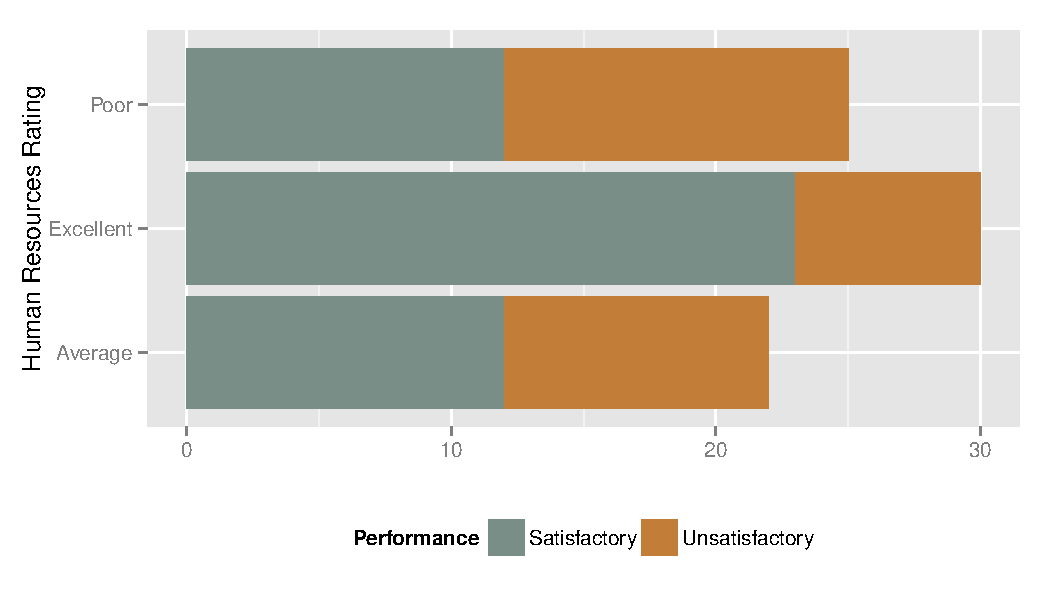
\includegraphics[width=\maxwidth]{figure/unnamed-chunk-5-1} 

}



\end{knitrout}

\end{frame}


\begin{frame}[fragile]
\begin{knitrout}
\definecolor{shadecolor}{rgb}{0.969, 0.969, 0.969}\color{fgcolor}\begin{kframe}
\begin{verbatim}
## 
## 	Pearson's Chi-squared test
## 
## data:  M
## X-squared = 5.2582, df = 2, p-value = 0.07214
\end{verbatim}
\end{kframe}
\end{knitrout}

\begin{itemize}
  \item<1-> H$_0$: There is no association between HR rating and job performance
  \item<2-> Probably need to intervene with HR!
\end{itemize}
\end{frame}


\frame{
\frametitle{Construct Validity}
\begin{itemize}
	\item Evidence supporting that the test \textit{measures} the underlying construct and that it is capable of \textit{placing} test takers along that latent construct 
	\item A test maker MUST have theories about the construct, it's definition, structure, and relationship to other constructs and has theories about how their test relates to other tests
	\item If the test fails to discern test takers, need to know \textcolor{wared}{why}
	  \begin{itemize}
	    \item Recall all the various potential sources of error in testing
	  \end{itemize}
	\item All forms of validity could be considered subsets of construct validity 
\end{itemize}
}

\frame{
\frametitle{Construct Validity Evidence}
\begin{itemize}
	\item \textcolor{wared}{Homogeniety}
		\begin{itemize}
			\item Structure of a test should be homogeneous if it is measuring a single construct
			\item Responses to test items should be positively correlated with total score on the test
			  \begin{itemize}
			    \item What kind of correlation is this?
			    \item Items that are not ... need to be removed or rewritten
			    \item What to do with items that have low correlations?
			    \item What does it mean to throw away items and rewrite them?
			  \end{itemize}
			\item Homogeneity implies inter item agreement ... how can we measure this?
		\end{itemize}
	\item<2-> Change with \textcolor{wared}{age} and \textcolor{wared}{pre/post}
		\begin{itemize}
			\item<2-> Testtakers taking a test in reading \textit{should} score higher on comprehension if they are older
			\item<2-> Students getting tutored in reading between a pre and post test should score higher on the post test
			\item<2-> Should we be able to predict how anxiety will change as we get older? 
		\end{itemize} 
\end{itemize}
}

\frame{
\frametitle{Construct Validity Evidence - contd}
\begin{itemize}
	\item<1-> Groups higher on the measured construct should have higher scores (\textcolor{wared}{method of contrasted groups})
		\begin{itemize}
			\item<1-> Administer a test measuring tendency toward violent behavior
			\item<1-> Who should have higher scores: The general public or prison inamtes for assault and battery?
		\end{itemize}
	\item<2-> \textcolor{wared}{Convergent} - Test takers IQ scores on a new test should be correlated with their IQ score from an established and validated IQ tests (or a related construct)
	\item<3-> \textcolor{wared}{Discriminant} - Test scores should be unrelated to scores from another instrument
	    \begin{itemize}
	      \item<3-> Ask students to score each other on leadership
	      \item<3-> Ask students to score each other on popularity
	      \item<3-> What does it mean if these two are uncorrelated?
	    \end{itemize}
\end{itemize}
}

\frame{
\frametitle{Factor Analysis}
\centerline{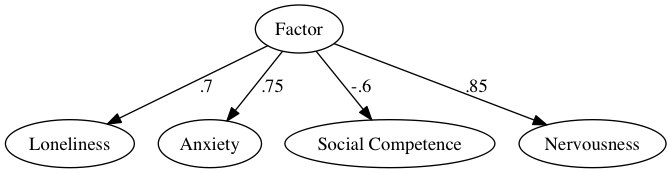
\includegraphics[scale=.5]{images/factor.png}}
\begin{itemize}
\item What should we call this factor?
\item If Nervousness is our new instrument to measure the factor, how well does it do?
\item What does it mean that social competence is negatively correlated with our factor?
\end{itemize}
}

\frame{
\frametitle{Test Bias and Fairness}
\begin{itemize}
	\item Test bias - degree to which a test systematically favors one group or another
	\begin{itemize}
		\item Can test for this statistically using logistic regression model
		\item  Known as \textcolor{wared}{differential item functioning}
		\item Errors by raters - too lightly, too severely, to the middle, too perfectly
	\end{itemize}
	\item Test fairness - the degree to which a test is fair and used in an equitable way
		\begin{itemize}
			\item What if we administer a test to a group not involved in the validation sample
			\item Maybe some groups of people are just different?
		\end{itemize}
	\item \textcolor{wared}{Why do we care about bias and fairness?}
\end{itemize}
}

\end{document}


